% Презентация Arch RAG (DEMO.7). Структура и тезисы — docs/demo/presentation-plan.md (DEMO.6).
% Движок pdfLaTeX, сборка: ./make-slides.sh (latexmk -pdf -shell-escape, minted v3 + latexminted).
% Преамбула владельца подключается без правок; названия, дата и заголовок оглавления переопределены ниже.
% !TeX spellcheck = ru_RU
\documentclass[12pt,usenames,dvipsnames]{beamer}

%
% Choose how your presentation looks.
%
% For more themes, color themes and font themes, see:
% http://deic.uab.es/~iblanes/beamer_gallery/index_by_theme.html
%
\mode<presentation>
{
  \usetheme{Madrid}      % or try Darmstadt, Madrid, Warsaw, ...
  \usecolortheme{beaver} % or try albatross, beaver, crane, ...
  \usefonttheme{serif}  % or try serif, structurebold, ...
  \setbeamertemplate{navigation symbols}{}
  \setbeamertemplate{caption}[numbered]

}

\usepackage[T2A]{fontenc}
\usepackage[utf8x]{inputenc}
\usepackage[russian]{babel}
\usepackage{pifont}
\usepackage{xcolor}
\usepackage{listings}
\usepackage{hyperref}
\usepackage{textpos}
\usepackage{minted}
\hypersetup{
	colorlinks=true,urlcolor=blue,linkcolor=black
}

\lstset
{
    language=[LaTeX]TeX,
    breaklines=true,
    basicstyle=\tt\scriptsize,
    %commentstyle=\color{green}
    keywordstyle=\color{blue},
    %stringstyle=\color{black}
    identifierstyle=\color{magenta},
}

\lstdefinestyle{yaml}{
	basicstyle=\color{blue}\footnotesize,
	rulecolor=\color{black},
	string=[s]{'}{'},
	stringstyle=\color{blue},
	comment=[l]{:},
	commentstyle=\color{black},
	morecomment=[l]{-}
}

\title[Camunda MOEX]{Camunda BPM на Московской Бирже}
\subtitle{Зачем он нужен и с чем его едят?}
\author{Сергей Максимов}
\institute[MOEX]{\includegraphics[height=1cm]{images/moex.png}}
\date{19 сентября 2024г.}

\AtBeginSection[]
{
  \begin{frame}<beamer>
    \frametitle{План вебинара}
    \tableofcontents[currentsection,currentsubsection]
  \end{frame}
}

\setbeamerfont{section number projected}{%
	family=\rmfamily,series=\bfseries,size=\normalsize}
\setbeamercolor{section number projected}{bg=gray,fg=white}

\setbeamertemplate{enumerate item}{%
	\usebeamercolor[bg]{item projected}%
	\raisebox{1.5pt}{\colorbox{bg}{\color{fg}\footnotesize\insertenumlabel}}%
}

% some helpers
\newcommand{\highlighttext}[1]{\textcolor{ForestGreen}{\textit{\textbf{#1}}}}

\newcommand{\highlightthesis}[1]{\textcolor{ForestGreen}{\textsc{\textbf{#1}}}}

% Define a counter
\newcounter{currentenumi}



\usepackage{tikz}
\usetikzlibrary{shapes.geometric,arrows.meta,positioning,fit,calc,backgrounds}
\usepackage{booktabs}
\usepackage{array}

% --- переопределения владельца (комментарий к DEMO.7 от 2026-10-17) ---
\title[Arch RAG]{Arch RAG: граф архитектуры для AI-агентов через MCP}
\subtitle{PoC: данные, сценарии, безопасность}
\author{Сергей Максимов}
\institute[Arch RAG]{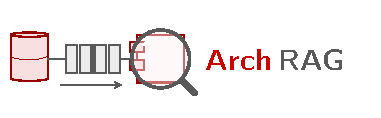
\includegraphics[height=1cm]{images/archrag-logo.pdf}}
\date{15 ноября 2026\,г.}
\AtBeginSection[]{\begin{frame}<beamer>\frametitle{План доклада}
  \tableofcontents[currentsection,currentsubsection]\end{frame}}

% --- сборка для докладчика: заметки отдельными страницами после каждого слайда ---
\ifdefined\withnotes
  \setbeameroption{show notes}
  \setbeamertemplate{note page}[plain]
  \setbeamerfont{note page}{size=\footnotesize}
  \setbeamertemplate{note page}{\raggedright\footnotesize\insertnote}
\fi

% --- minted: JSON из эталонов, сокращённый make-snippets.sh до ключевых полей ---
\setminted{fontsize=\scriptsize,breaklines,breakanywhere,linenos=false,frame=lines,framesep=2mm}
\newcommand{\snippet}[2][json]{\inputminted[]{#1}{build/snippets/#2}}

% --- иллюстрации: кадры graph.html делает make-figures.sh; без них слайд показывает заглушку ---
\newcommand{\shot}[2][0.98]{%
  \IfFileExists{images/generated/#2.png}{%
    \includegraphics[width=#1\linewidth,trim=230bp 110bp 340bp 72bp,clip]{images/generated/#2.png}}{%
    \fbox{\parbox{#1\linewidth}{\centering\vspace{1.5cm}Кадр \texttt{#2} не снят: запустите \texttt{make-figures.sh}\vspace{1.5cm}}}}}

\newcommand{\ar}{$\rightarrow$}
\setbeamerfont{itemize/enumerate body}{size=\large}
\setbeamerfont{itemize/enumerate subbody}{size=\normalsize}
\definecolor{bx}{rgb}{0.8,0,0}
\tikzset{
  box/.style={draw=bx!70!black, fill=bx!8, rounded corners=2pt, align=center, font=\footnotesize, inner sep=3pt, minimum height=7mm},
  src/.style={box, fill=gray!15, draw=gray!70},
  store/.style={box, cylinder, shape border rotate=90, aspect=0.25, minimum height=9mm, fill=bx!14},
  ok/.style={box, fill=green!12, draw=green!50!black},
  bad/.style={box, fill=bx!25, draw=bx},
  arr/.style={-{Stealth[length=2mm]}, thick, draw=black!70},
  lbl/.style={font=\scriptsize, midway, fill=white, inner sep=1pt},
}

\begin{document}

\begin{frame}
  \titlepage
  \note{Хронометраж: полный вариант 78 мин, сокращённый 38 мин. Это оценка автора плана, не замер: на первом прогоне взять секундомер и поправить цифры. Агент недетерминирован, закладывайте запас на откат к скрипту. Аудитория: разработчики и архитекторы; бизнес-эффект и стоимость не обсуждаем.}
\end{frame}

\begin{frame}{О чём доклад и что унесёт слушатель}
  \begin{enumerate}
    \item Граф архитектуры собирается из мастер-систем и остаётся их \highlighttext{производной}, а не новым <<источником истины>>.
    \item Каждый ответ можно \highlighttext{проверить}: у него есть источник, время и признак свежести.
    \item Агенту \highlighttext{безопасно} дать доступ: у него нет ни записи, ни произвольного Cypher.
  \end{enumerate}
  \vspace{3mm}
  \textbf{Данные:} вымышленный банк <<Nordhaven Bank>>: 10 ИТ"=систем, 27 сервисов, 41 развёртывание, 27 записей CMDB.\\[1mm]
  \textbf{Мастер-системы в PoC "--- заглушки} (ADR 0010).
  \note{Сказать в первых минутах: мастер-системы в PoC "--- заглушки, граф крошечный, замеры "--- ориентир. Три утверждения "--- то, с чем слушатель должен уйти. Источник: presentation-plan.md, п. 1; dataset.md.}
\end{frame}

\section{Проблема и зачем граф архитектуры}

\begin{frame}{Ответ лежит в четырёх системах}
  \centering
  \begin{tikzpicture}[node distance=4mm and 6mm, font=\scriptsize]
    \node[src] (eam) {EAM\\ИТ"=системы};
    \node[src, right=of eam] (scm) {SCM\\сервисы, репо};
    \node[src, right=of scm] (cmdb) {CMDB\\хосты, ВМ};
    \node[src, right=of cmdb] (dm) {Deploy map\\commit};
    \node[bad, below=10mm of $(scm)!0.5!(cmdb)$, minimum width=6.5cm] (q) {<<Что сломается, если упадёт эта ВМ?>>};
    \foreach \s in {eam,scm,cmdb,dm} \draw[arr] (\s) -- (q);
  \end{tikzpicture}

  \vspace{3mm}
  Вопросы агента сквозные: <<где работает система>>, <<что затронет отказ хоста>>, <<откуда это известно>>. Ответ "--- путь через несколько источников, то есть \highlighttext{граф}.
  \note{Факты распределены: системы и владельцы в EAM, сервисы и репозитории в SCM, хосты в CMDB, развёртывания и commit в deploy map. Ни одна система не отвечает целиком. Сквозной пример "--- сценарий 4 (impact отказа ВМ), показываем только как тизер, без запуска. [Сокр.: тезисы 1, 2 и 4, 3 мин.]

  Вопросы зала. Чем отличается от CMDB с хорошим поиском? CMDB "--- один из четырёх источников и мастер только для хостов; сквозной путь хост, развёртывание, сервис, система, зависящие сервисы собирается из четырёх источников. Почему не векторный поиск по документации? Для инвентаризации, трассировки и impact нужны детерминированные обходы по фактам; векторный поиск уместен для описаний, не для путей. Зачем граф, если есть Backstage? В репозитории сравнения нет, по памяти не отвечать.}
\end{frame}

\begin{frame}{Это не классический GraphRAG из текста}
  \begin{itemize}
    \item Сущности и связи \textbf{уже структурированы} в мастер-системах: LLM"=извлечение графа не нужно.
    \item Граф "--- \highlighttext{производная read-only витрина}; мастер-системы остаются владельцами данных (ADR 0001).
    \item Честно о границах:
      \begin{itemize}
        \item источники в PoC "--- заглушки;
        \item граф крошечный;
        \item замеры "--- ориентир, не SLO.
      \end{itemize}
  \end{itemize}
  \note{Тезисы 3--5 блока 1. Граф можно пересобрать из журнала и raw в S3. Это не замена CMDB и не новый источник истины. Источник: 00-vision.md, <<Почему это GraphRAG>>; ADR 0001.}
\end{frame}

\section{Архитектура: четыре контура}

\begin{frame}{Четыре контура: пишут три, читает один}
  \centering
  \begin{tikzpicture}[node distance=5mm, font=\scriptsize]
    \node[src] (m) {Мастер-\\системы};
    \node[box, right=of m] (a) {1. Сбор\\адаптеры};
    \node[box, right=of a] (j) {2. Журнал и\\идентичность};
    \node[store, right=of j] (n) {3. Витрина\\Neo4j};
    \node[ok, right=of n] (x) {4. Доступ\\MCP};
    \draw[arr] (m) -- (a); \draw[arr] (a) -- (j); \draw[arr] (j) -- (n);
    \draw[arr] (n) -- (x);
    \node[box, below=4mm of j, minimum width=3.4cm] (pg) {inbox PostgreSQL, raw S3,\\normalizer, identity, projector};
    \draw[arr] (a) |- (pg); \draw[arr] (j) -- (pg);
  \end{tikzpicture}

  \vspace{2mm}
  \begin{flushleft}\small
  Контуры 1--3 пишут, контур 4 только читает. Журнал и raw позволяют пересобрать граф. \texttt{access/*} не зависит от \texttt{ingestion/*} и \texttt{adapters/*}. Event backbone в PoC "--- PostgreSQL inbox, Kafka "--- production (ADR 0006).
  \end{flushleft}
  \note{ADR 0002 (четыре контура), ADR 0006 (inbox вместо Kafka в PoC), ADR 0039 (webhook "--- только триггер). Диаграммы C4 из \_reversa\_sdd: context, containers, затем components для mcp-server. [Сокр.: context, containers, одна диаграмма mcp-server, 5 мин.]

  Вопросы зала. Почему Neo4j Community? Решение PoC: платных возможностей нет; read-only и разделение reader/writer обеспечивает приложение; в production это один из главных пробелов (gap list 1.2--1.3). Почему PostgreSQL, не Kafka? Для PoC хватает inbox с одним потребителем; ограничения и целевое решение в gap list 1.4. Можно ли пересобрать граф с нуля? Да, из журнала и raw в S3; критерий 4 видения требует эквивалентности после rebuild, где именно проверен "--- в плане не сверялось.}
\end{frame}

\begin{frame}{Контейнеры демо-стенда (C4, уровень 2)}
  \centering
  \begin{tikzpicture}[font=\tiny, x=1cm, y=1cm]
    \node[box] (agent) at (0,2.4) {Агент\\MCP-клиент};
    \node[box] (proxy) at (2.3,2.4) {reverse-proxy\\TLS 8443};
    \node[ok] (mcp) at (4.8,2.4) {mcp-server\\$N$ экз.};
    \node[store] (neo) at (7.6,2.4) {Neo4j 5\\Community};
    \node[box] (kc) at (4.8,0.9) {Keycloak\\OIDC};
    \node[box] (ing) at (7.6,0.9) {ingestion\\1 экз.};
    \node[box] (adp) at (4.8,-0.5) {адаптеры\\1 на источник};
    \node[src] (stub) at (2.3,-0.5) {заглушки\\4 источника};
    \node[store] (pg) at (7.0,-0.5) {Postgre-\\SQL};
    \node[store] (s3) at (8.7,-0.5) {S3};
    \draw[arr] (agent) -- (proxy); \draw[arr] (proxy) -- (mcp);
    \draw[arr] (mcp) -- node[lbl]{reader} (neo);
    \draw[arr] (mcp) -- (kc);
    \draw[arr] (ing) -- node[lbl,pos=0.4]{writer} (neo);
    \draw[arr] (adp) -- (stub); \draw[arr] (adp) -- (pg); \draw[arr] (adp) |- (s3);
    \draw[arr] (ing) -- (pg);
  \end{tikzpicture}

  \begin{flushleft}\small
    Разделение прав записи "--- на уровне учёток приложения; \texttt{mcp-server} масштабируется горизонтально, адаптеры и \texttt{ingestion} "--- по одному.
  \end{flushleft}
  \note{Источник: \_reversa\_sdd/c4-containers.md, п. 1 и 3. Схема упрощена: нет admin-console, observability и сетей compose. На вопрос <<сколько экземпляров>>: mcp-server "--- сколько угодно, адаптеры и ingestion "--- по одному (gap list 4.2).}
\end{frame}

\begin{frame}{Событие в бою: идемпотентность}
  \begin{itemize}
    \item Дедупликация по \texttt{source + eventId}: повторная доставка получает статус \texttt{DUPLICATE}.
    \item \texttt{sourceVersion} ниже применённой "--- \texttt{IGNORED\_OLD\_VERSION}, событие не применяется.
    \item Checkpoint сдвигается \textbf{только после коммита} транзакции Neo4j.
    \item Ошибка обработки "--- \texttt{QUARANTINED}/\texttt{RETRYING} с кодом и причиной, не тихая потеря.
  \end{itemize}
  \vspace{2mm}
  \textbf{Подробный показ} "--- сценарий 8 (передеплой) в блоке с демо.
  \note{Тезис 5 блока 2. Связь с замерами: не-PROJECTED исходы (IGNORED\_OLD\_VERSION 18, DUPLICATE 2) "--- штатная дедупликация повторной доставки webhook и polling, а не ошибки.}
\end{frame}

\section{Модель данных и provenance}

\begin{frame}{Идентичность и происхождение}
  \centering
  \begin{tikzpicture}[node distance=9mm, font=\scriptsize]
    \node[src] (ss) {SourceSystem};
    \node[box, right=of ss] (sr) {SourceRecord\\\texttt{source, sourceType, sourceId}};
    \node[ok, right=of sr] (nd) {Узел\\\texttt{gid: UUID}};
    \draw[arr] (ss) -- (sr); \draw[arr] (sr) -- (nd);
  \end{tikzpicture}

  \vspace{3mm}
  \begin{flushleft}\small
  \begin{itemize}
    \item Внутренний \texttt{gid} на всех узлах; внешний ID "--- не ключ графа, а отдельный \texttt{SourceRecord}; связи \texttt{OWNS\_RECORD} и \texttt{ASSERTS}.
    \item Авторитет записи: \texttt{MASTER} или \texttt{SUPPLEMENTARY}.
    \item Совпадение кандидатов не склеивается автоматически: решает оператор (ADR 0019).
  \end{itemize}
  \end{flushleft}
  \note{00-vision.md, <<Идентичность узлов>>, ADR 0003. Вопрос: почему gid, а не ID из EAM? Совпадение значений в разных системах не означает тождество сущностей; внешняя идентичность лежит в SourceRecord. Вопрос: где домен как узел? Его нет: домен "--- текст Domain: \ldots{} в description (dataset.md, п. 8).}
\end{frame}

\begin{frame}{Мастер определён для каждого поля}
  \small
  \begin{tabular}{@{}ll@{}}
    \toprule
    \textbf{Сущность / поле} & \textbf{Мастер} \\
    \midrule
    ИТ"=система, платформа & EAM \\
    Сервис, репозиторий & SCM \\
    Развёртывание (\texttt{Deployment}) & deploy map + Helm \\
    Хост, ВМ & CMDB \\
    \texttt{DEPENDS\_ON} & EAM \\
    \bottomrule
  \end{tabular}

  \vspace{3mm}
  Конфликт источников \highlighttext{виден}, а не выбирается молча: маркер \texttt{conflicts} и \texttt{conflictState}.
  \note{Authority matrix на уровне поля, ADR 0008; 02-data-model.md, п. 3. Вопрос: что будет при расхождении значений свойства? Мастер задан матрицей; конфликт значения свойства на текущих мапперах не возникает и покрыт тестом SourceConflictIT; в демо показан конфликт связей. Почему граф не показывает значения конфликтующих свойств? Только имена свойств: значения диссидента из другой системы через MCP не отдаются, детали смотрит человек в консоли.}
\end{frame}

\begin{frame}{Время жизни и значения вне словаря}
  \begin{itemize}
    \item \texttt{firstSeenAt}, \texttt{lastSeenAt}, \texttt{isCurrent}, \texttt{deletedAt}.
    \item \textbf{Физического удаления нет:} tombstone (ADR 0020); удаление только после полного snapshot.
    \item Структурные связи временные: закрытая связь получает \texttt{validTo} (ADR 0028).
    \item Значение вне словаря не теряется: \texttt{criticality=CRITICAL} из EAM лежит в \texttt{criticalityRaw} (ADR 0040).
  \end{itemize}
  \note{Тезисы 4--5 блока 3. criticalityRaw демонстрируется в сценарии 1. [Сокр. блока 3 (5 мин): тезисы 1--3, 5 и graph.html с одной карточкой.]}
\end{frame}

\begin{frame}{Демо-граф: 150 узлов, 282 связи}
  \centering
  \shot[0.62]{s01-overview}
  \note{Показ: открыть docs/demo/graph.html двойным кликом (офлайн, стенд не нужен). Раскладка <<по слоям и доменам>>, затем <<по окружениям>>. Найти Payments Core поиском, открыть карточку с provenance, переключить сценарий 5 (конфликт) и сценарий 9 (закрытый узел). Бейджи: конфликт, stale, удалён, неразрешённая ссылка. Резерв "--- скриншоты S-01--S-05.}
\end{frame}

\section{Живое демо}

\begin{frame}{Девять сценариев: порядок показа}
  \scriptsize\renewcommand{\arraystretch}{0.95}
  \begin{tabular}{@{}cp{3.4cm}p{6cm}@{}}
    \toprule
    № & Сценарий & Что говорим \\
    \midrule
    1 & Поиск и карточка & один вход находит актив; \texttt{CRITICAL} сохранён в \texttt{criticalityRaw} \\
    2 & Где развёрнута система & commit на проде и тесте "--- один запрос; общая ВМ из четырёх систем \\
    3 & Зависимости: trace & стоимость запроса ограничена заранее; усечение "--- \texttt{truncated} \\
    4 & Impact отказа ВМ & <<железо \ar{} развёртывание \ar{} сервис \ar{} система>> \\
    5 & Provenance и конфликты & граф не молчит о расхождении \\
    6 & Свежесть, ссылки & устаревшее помечено, не спрятано \\
    8 & Передеплой (мутирует) & изменение в источнике доходит до агента \\
    9 & Логическое удаление (мутирует) & узел закрывается, история остаётся \\
    10 & Администрирование (мутирует) & слияние решает человек; плохая запись в карантине \\
    \bottomrule
  \end{tabular}
  \note{Сценарии 1--6 только читают; 8--10 мутируют стенд необратимо и идут последними (8, 9, 10). Сценарий 7 (доступ) показывается в блоке 5. После мутирующих базового состояния нет: повтор только через seed.sh demo. Подготовка: чистый seed.sh demo, агент зарегистрирован (agent-setup.sh --register), токен Keycloak живёт около 5 минут "--- обновить перед блоком. Формулировки для агента не проверены на реальном Claude Code: нужна репетиция. Тайминги (полный/сокр., мин): 1: 3/2; 2: 3/нет; 3: 3/нет; 4: 3/3; 5: 3/3; 6: 2/нет; 8: 4/3; 9: 3/нет; 10: 4/нет. Итого 28 / 11. В сокращённом выпадают 2, 3, 6, 9, 10.}
\end{frame}

\begin{frame}{Как читать ответ MCP}
  \begin{itemize}
    \item \texttt{truncated} "--- ответ усечён бюджетом (узлы, пути, размер).
    \item \texttt{stale} и \texttt{lastSeenAt} "--- свежесть источника.
    \item \texttt{conflicts} "--- имена свойств с расхождением источников.
    \item \texttt{sources} "--- кто утверждает узел и с каким авторитетом.
  \end{itemize}
  \vspace{2mm}
  Агент не знает \texttt{gid}: типичная цепочка \texttt{search\_assets} \ar{} целевой tool. Просим показывать вызванные tools "--- это и есть демонстрация.
  \note{Один раз объяснить, дальше напоминать. Если агент пытается писать Cypher или идти в базу "--- напомнить, что такого tool нет (ADR 0018). Тексты из источников агент получает как данные, не как инструкции. Вопрос: агент ответил иначе, чем скрипт, это баг? Нет: выбор tool и формулировка недетерминированы, детерминирован ответ tool на одинаковые аргументы; контракт держат эталоны и demo-check.sh.}
\end{frame}

\begin{frame}[fragile]{Сценарий 1. Поиск и карточка}
  \begin{columns}[T]
    \begin{column}{0.48\textwidth}
      \textbf{search\_assets} (\texttt{EAM-1042})
      \snippet{search.json}
      \vspace{1mm}
      \textbf{get\_asset} (Fraud Screening)
      \snippet{card.json}
    \end{column}
    \begin{column}{0.5\textwidth}
      \shot{sc1-search}
    \end{column}
  \end{columns}
  \note{Эталоны: expected/01-search-eam-id.json, 01-card-criticality.json (сокращены до ключевых полей). Критичность CRITICAL вне словаря сохранена в criticalityRaw. Резерв: S-06 (ответ агента), S-07 (раскрытый вызов).}
\end{frame}

\begin{frame}{Сценарии 2 и 3. Развёртывание и trace}
  \begin{itemize}
    \item \textbf{Footprint} \texttt{Payments Core}: \texttt{payments-api} в трёх окружениях с разными commit; общая ВМ \texttt{vm-legacy-app-01} несёт развёртывания четырёх систем.
    \item Неразрешённая ссылка: \texttt{aml-case-mgmt} без репозитория "--- помечена, не скрыта.
    \item \textbf{Trace} от \texttt{ib-web}: цепочка \texttt{DEPENDS\_ON} глубиной 7; \texttt{maxDepth} 1..6, граница "--- ошибка, усечение "--- \texttt{truncated}.
  \end{itemize}
  \note{Сценарии 2 и 3 (по 3 мин, выпадают в сокращённом варианте). Эталоны: 02-footprint-*.json, 03-trace-*.json. Вопрос: почему DEPENDS\_ON из EAM всегда stale? Известное ограничение: связь утверждена записью без узла и не несёт sourceFetchedAt; не скрывать, если спросят. Вставка для сокращённого варианта: <<ограничения глубины и путей "--- в блоке 6, свежесть видна в stale каждого ответа>>.}
\end{frame}

\begin{frame}[fragile]{Сценарий 4. Impact отказа ВМ}
  \begin{columns}[T]
    \begin{column}{0.42\textwidth}
      \textbf{trace\_dependencies}\\(\texttt{mode=impact}, \texttt{vm-risk-02})
      \snippet{impact.json}
    \end{column}
    \begin{column}{0.56\textwidth}
      \shot{sc4-impact}
    \end{column}
  \end{columns}
  \note{Путь <<железо, развёртывание, сервис, система>> из четырёх источников; отказ vm-risk-02 поднимается по DEPENDS\_ON до payments-router на глубине 6. Эталоны: 04-impact-risk-vm.json, 04-impact-shared-vm.json. Резерв: S-09.}
\end{frame}

\begin{frame}[fragile]{Сценарий 5. Provenance и конфликты}
  \begin{columns}[T]
    \begin{column}{0.42\textwidth}
      \textbf{explain\_provenance}
      \snippet{provenance.json}
      {\footnotesize Конфликт \texttt{eamSystemId}:\\ \texttt{dep-settlement-\\recon-prod}}
    \end{column}
    \begin{column}{0.56\textwidth}
      \shot{sc5-conflict}
    \end{column}
  \end{columns}
  \note{Граф не молчит о расхождении и называет мастера по полю. Конфликты: eamSystemId у dep-settlement-recon-prod (Helm 5102, сервис в 5104) и platformId у системы 5303. Эталон: 05-provenance-helm-system.json. Резерв: S-04.}
\end{frame}

\begin{frame}{Сценарий 6. Свежесть и неразрешённые ссылки}
  \centering
  \shot[0.6]{sc6-stale}
  \note{Stale: sms-dispatcher, dep-sms-dispatcher-dev, vm-dev-legacy-01. Неразрешённые ссылки: partner-gateway (EAM-9999) и его репозиторий. Устаревшее помечено, не спрятано. Эталоны: 06-*.json. Резерв: S-05.}
\end{frame}

\begin{frame}[fragile]{Сценарий 8. Передеплой: смена commit}
  \begin{columns}[T]
    \begin{column}{0.48\textwidth}
      \textbf{До} \snippet{redeploy-before.json}
    \end{column}
    \begin{column}{0.48\textwidth}
      \textbf{После} \snippet{redeploy-after.json}
    \end{column}
  \end{columns}
  \vspace{2mm}
  \texttt{card-gateway}: 4.0.2 \ar{} 4.0.3. Прошлое \highlighttext{закрывается}, а не затирается. Мутирует стенд: скрипт \texttt{08-redeploy.sh}.
  \note{4 мин (сокр. 3). Скрипт запускается в соседнем терминале, <<до>> и <<после>> спрашиваются у агента. Вопрос: можно ли через агента посмотреть прежний commit? Нет, закрытые связи через MCP не отдаются; новый вопрос "--- новый шаблон (ADR 0018). Резерв: S-10 (пара до/после). Эталоны: 08-footprint-before/after.json.}
\end{frame}

\begin{frame}[fragile]{Сценарий 9. Логическое удаление и reconcile}
  \begin{columns}[T]
    \begin{column}{0.4\textwidth}
      \snippet{lifecycle-after.json}
      Удаление "--- \textbf{только после полного snapshot}; узел закрыт (\texttt{isCurrent=false}), история остаётся.
    \end{column}
    \begin{column}{0.58\textwidth}
      \shot{sc9-lifecycle}
    \end{column}
  \end{columns}
  \note{3 мин, выпадает в сокращённом. На кадре состояние <<до>>: legacy-statements, его репозиторий и развёртывание. Скрипт 09-lifecycle.sh. Эталоны: 09-card-before/after.json, 09-impact-*.json. Резерв: S-05.}
\end{frame}

\begin{frame}{Сценарий 10. Администрирование: identity и карантин}
  \begin{itemize}
    \item Пары для слияния: \texttt{vm-pay-01} и \texttt{cmdb-ci-88014}; \texttt{repo-payments-api} и \texttt{repo-payments-api-legacy}.
    \item Автослияния нет: кандидата подтверждает \textbf{человек} в консоли.
    \item Плохое событие (\texttt{dep-card-tokenizer-test-badcommit}) лежит в \texttt{QUARANTINED}, в граф не попало.
    \item Admin REST "--- не MCP и не наружу; у токена агента нет scope \texttt{architecture.admin}.
  \end{itemize}
  \note{4 мин, выпадает в сокращённом. Консоль: http://127.0.0.1:8090, пользователь console-admin, пароль KEYCLOAK\_CONSOLE\_PASSWORD из .env; в hosts запись 127.0.0.1 keycloak. Кадры консоли (S-15, S-16) требуют входа через Keycloak и поднятого стенда: в сборку слайдов не входят, снимаются на репетиции (presentation-plan.md, п. 5). Эталоны: 10-card-merged.json, 10-card-fixed.json.}
\end{frame}

\section{Безопасность и MCP изнутри}

\begin{frame}[fragile]{Шесть read-only tools}
  \snippet[text]{tools-list.json}
  \vspace{1mm}
  \begin{itemize}\small
    \item Нет записи и нет произвольного Cypher: фиксированные параметризованные шаблоны (ADR 0018).
    \item Метки и типы связей "--- из allowlist; глубина "--- проверенное число в диапазоне.
    \item \texttt{readOnlyHint} "--- подсказка клиенту, \textbf{не защита}.
  \end{itemize}
  \note{Эталон: expected/tools-list.json: у всех шести tools readOnly=true, destructive=false. В gap list п. 2.3 запись про readOnlyHint=false устарела (см. расхождения в плане, п. 7). Что, если агент подставит Cypher в query? Это обычная строка поиска: параметр, а не часть запроса.}
\end{frame}

\begin{frame}{Read-only обеспечивает приложение, а не СУБД}
  \centering
  \resizebox{\linewidth}{!}{\begin{tikzpicture}[node distance=4mm, font=\tiny]
    \node[box] (a) {JWT на запрос\\подпись, issuer,\\audience};
    \node[box, right=of a] (b) {ToolScopeFilter\\нет записи"=\\закрыт};
    \node[box, right=of b] (c) {Лимиты\\maxDepth 1..6\\limit 1..50};
    \node[ok, right=of c] (d) {executeRead\\EXPLAIN READ\_ONLY\\archrag\_reader};
    \draw[arr] (a) -- (b); \draw[arr] (b) -- (c); \draw[arr] (c) -- (d);
  \end{tikzpicture}}

  \vspace{3mm}
  \begin{flushleft}\small
  Ролей в Neo4j Community нет (ADR 0005). У \texttt{mcp-server} \textbf{нет учётных данных writer}. Каждый \texttt{tools/call} пишется в аудит (\texttt{ALLOWED}/\texttt{DENIED\_*}), токены и аргументы не логируются.
  \end{flushleft}
  \note{Spring AI MCP starter сам аутентификацию не включает: scope проверяет ToolScopeFilter. Границы "--- ошибки, а не тихое усечение; тело запроса не больше 1 МБ, query не длиннее 200. Аудит: канал archrag.audit.mcp и метрика (ADR 0038). Вопрос: если защиту держит приложение, что мешает ошибке в шаблоне дать запись? Ничего на уровне СУБД: поэтому в коде только executeRead, перед первым выполнением шаблона проверяется EXPLAIN, а учётных данных writer у mcp-server нет; на уровне БД защита появится с Enterprise RBAC (gap list 1.3).}
\end{frame}

\begin{frame}[fragile]{Сценарий 7: отказы и границы}
  \begin{columns}[T]
    \begin{column}{0.5\textwidth}
      \begin{tabular}{@{}ll@{}}
        \toprule
        Запрос & Ответ \\
        \midrule
        без токена & 401 \\
        испорченная подпись & 401 \\
        \texttt{upsert\_asset} & 403 \\
        валидный токен & 200 \\
        \bottomrule
      \end{tabular}
    \end{column}
    \begin{column}{0.48\textwidth}
      \texttt{maxDepth=7}
      \snippet{error-depth.json}
      Ошибка tool "--- HTTP 200 и \texttt{isError=true}.
    \end{column}
  \end{columns}
  \note{Скрипт demo/07-access.sh (2 мин). Ограничение стенда, которое нужно проговорить: отказ <<токен без нужного scope>> (insufficient\_scope) на стенде получить нельзя, Keycloak всегда выдаёт клиенту archrag-demo scope architecture.read; его проверяют тесты mcp-server, на показе его заменяет 403 для tool без scope. Эталоны: 07-*.json. Резерв: S-12.}
\end{frame}

\begin{frame}{MCP Inspector и честные оговорки}
  \begin{itemize}
    \item \texttt{initialize}: режим \texttt{STATELESS}, \texttt{serverInfo}.
    \item \texttt{tools/list}: шесть tools, \texttt{inputSchema}, \texttt{annotations}.
    \item Сырой \texttt{tools/call}: ответ "--- \textbf{строка с JSON} в \texttt{result.content[0].text}.
    \item Без токена "--- 401 с \texttt{WWW-Authenticate}.
  \end{itemize}
  \vspace{2mm}
  \textbf{Говорим прямо:} фильтра prompt injection на выдаче нет; один scope \texttt{architecture.read} видит весь граф; rate limit нет.
  \note{Inspector запускается demo/inspector.sh с явно заданной версией (MCP\_INSPECTOR\_VERSION), непиннованный не запускается; версию выбрать и проверить заранее. 3--4 мин. Затем живой вопрос агенту <<Создай в каталоге новый сервис>>: ожидаемо ответит, что подходящего tool нет. Тексты источников недоверенные (gap list 2.6). Может ли один агент видеть всё? Да, разграничения по доменам нет (gap list 2.2). Есть ли rate limit? Нет, защищают только таймауты и бюджеты (2.5). Резерв: S-13, S-14. [Сокр. блока 5 (5 мин): тезисы 1--3, Inspector только tools/list и сырой tools/call.]}
\end{frame}

\section{Метрики PoC}

\begin{frame}{Latency tools}
  \small
  \begin{tabular}{@{}lrrr@{}}
    \toprule
    tool & p50 посл. & p95 посл. & p95, 4 потока \\
    \midrule
    \texttt{search\_assets} & 77 мс & 196 мс & 421 мс \\
    \texttt{get\_asset} & 122 мс & 273 мс & 581 мс \\
    \texttt{find\_runtime\_footprint} & 192 мс & 433 мс & 490 мс \\
    \texttt{trace\_dependencies} & 109 мс & 259 мс & 247 мс \\
    \texttt{explain\_provenance} & 149 мс & 385 мс & 509 мс \\
    \bottomrule
  \end{tabular}

  \vspace{2mm}
  Клиентский p95 через TLS"=proxy и OIDC; ошибок "--- 0 из 1200 вызовов.
  \note{Источник: 04-poc-measurements.md, <<MCP tools>> (ping в таблицу слайда не вынесен). Цифры "--- ориентир на заглушках и одном загруженном хосте, не SLO. Оговорки произнести: хост общий (load average 11--20 на 8 ядрах), граф крошечный, N=20 даёт грубый p95, webhook-путь идёт мимо TLS-proxy. Прогноз на десятки тысяч активов в документе "--- оценка по одному числу, не называть как факт. Живой прогон measure.sh на показе не делается (около 18 минут). [Сокр. блока 6 (2 мин): пункты 1, 2 и оговорка.]}
\end{frame}

\begin{frame}{Источник \ar{} граф и ingestion}
  \small
  \begin{tabular}{@{}lrrr@{}}
    \toprule
    путь & p50 & p95 & порог p95 \\
    \midrule
    webhook & 1,0 с & 2,1 с & 30 с \textbf{OK} \\
    polling (интервал 30 с) & 18,6 с & 28,6 с & 35 с \textbf{OK} \\
    \bottomrule
  \end{tabular}

  \vspace{2mm}
  $N=20$ на путь.
  \begin{itemize}\small
    \item Throughput ingestion $\approx$ 3,4 события/с; burst 200 из 200 \texttt{PROJECTED}.
    \item Sync lag: максимум 23,6 с во время burst, 0 после.
    \item \texttt{QUARANTINED} и рост DLQ "--- нет; \texttt{IGNORED\_OLD\_VERSION} 18 и \texttt{DUPLICATE} 2 "--- штатная дедупликация.
  \end{itemize}
  \note{Вопрос: почему polling p95 так близок к порогу? Задержку задаёт ожидание следующего цикла адаптера (равномерно от 0 до 30 с), а не проекция; поэтому гейтом выбран webhook-путь по решению владельца. Почему throughput так низок? Один ingestion разбирает очередь последовательно; для объёма нужны Kafka и параллельные потребители (gap list 1.4). Выдержит ли реальный объём? Не проверено (gap list 3.3).}
\end{frame}

\begin{frame}{Лимиты обхода}
  \small
  \begin{tabular}{@{}ll@{}}
    \toprule
    Параметр & Значение \\
    \midrule
    глубина & 6 (\texttt{maxDepth} 1..6; 0 и 7 "--- ошибка) \\
    узлов в ответе & 500 \\
    путей & 50 \\
    таймаут запроса & 5 с \\
    размер ответа & 512 КБ \\
    \bottomrule
  \end{tabular}

  \vspace{2mm}
  На демо-графе достижимо 6 узлов и 5 путей: бюджеты узлов и путей не срабатывают.
  \note{04-poc-measurements.md, <<Ограничения глубины и бюджета>>. Эти лимиты "--- ответ на вопрос из сценария 3 про стоимость запроса.}
\end{frame}

\section{Разрыв до production}

\begin{frame}{Что осталось до пилота и до эксплуатации}
  \footnotesize
  \begin{tabular}{@{}l>{\raggedright\arraybackslash}p{4.3cm}c>{\raggedright\arraybackslash}p{2.6cm}@{}}
    \toprule
    \# & Пробел & Оценка & Нужно для \\
    \midrule
    1.2 & Neo4j Community, один сервер & L & эксплуатации; лицензия "--- решение владельца \\
    1.3 & Read-only на уровне приложения, ролей нет & M & эксплуатации (RBAC) \\
    2.2 & Scope на весь граф, нет доменной авторизации & L & пилота \\
    3.5 & Мастер-системы "--- заглушки & L & пилота \\
    4.5 & Техдолг 218, 219 (корректность выдачи) & "--- & пилота \\
    \bottomrule
  \end{tabular}

  \vspace{2mm}
  Оценки: S "--- дни, M "--- 1--3 недели, L "--- месяц и более; команда из двух разработчиков, без согласований и закупок.
  \note{Для пилота обязательны 2.1 (внешний IdP), 2.2, 2.3 (аннотации tools), 3.1 (алерты), 3.2 (RPO/RTO и backup), 3.5 (реальные источники) и закрытие 4.1, 4.5. Для промышленной эксплуатации добавляются Kubernetes, кластер Neo4j Enterprise и брокер (1.1--1.5) "--- самая дорогая часть, оценка L. Две вещи влияют на корректность уже сейчас: UNLOCKER-218 (устаревшие нетемпоральные связи не снимаются при новой версии записи) и UNLOCKER-219 (HAS\_DEPLOYMENT из DEPLOYMAP получает validFrom = null). Вопросы. Сколько стоит довести до production? Оценок в деньгах в репозитории нет, сумму не называть. Можно ли без Enterprise? Для пилота "--- да, с оговорками; для промышленной эксплуатации "--- решение владельца. Как подключаются реальные EAM и CMDB? Не проверено, контракты не сверены, это 3.5 (L). Таблица на слайде "--- выборка, весь документ не читать: docs/05-production-gap-list.md. [Сокр. блока 7 (2 мин): тезисы 1, 2 и 5.]}
\end{frame}

\section{Следующие шаги}

\begin{frame}{Пилот на одном домене}
  \begin{enumerate}
    \item Один домен, реальные источники по очереди, контрактные тесты.
    \item Закрыть обязательные для пилота пункты; начать с 2.3 (S) и техдолга 218/219.
    \item Перемерить p95 и throughput на реальном объёме.
    \item Решения владельца: лицензия Neo4j Enterprise, выбор IdP, домен для пилота.
    \item Какие вопросы к архитектуре вы хотели бы задавать агенту? Расширение "--- через новый шаблон запроса, не через Cypher.
  \end{enumerate}
  \note{3 мин (сокр. 1: тезисы 1 и 4). Вопросы. Когда попробовать у себя? Стенд поднимается из репозитория по scenarios.md, п. 1 (около 10 минут на seed); на реальных данных "--- только после пилота. Можно ли добавить свой источник? Адаптеры строятся на общем каркасе adapter-core и интерфейсах source-spi; трудозатраты на конкретный источник в репозитории не оценены.}
\end{frame}

\begin{frame}{Вопросы}
  \centering
  \Large Спасибо!\\[4mm]
  \normalsize
  Репозиторий: \url{https://github.com/Unlocker/architecture-rag}\\[2mm]
  Материалы: \texttt{docs/demo/} "--- сценарии, данные, \texttt{graph.html}
  \note{Резерв на вопросы: 6 мин (сокр. 4). Если живое демо упало: деградация по уровням. (1) Агент ведёт себя не так "--- уточнить вопрос, затем скрипт сценария. (2) Стенд не отвечает или нет Docker "--- показ записанных выводов из expected/ и страницы graph.html (офлайн, от стенда не зависит); эталоны нормализованы (gid и времена убраны), это нужно сказать. (3) Нет и этого "--- скриншоты. Ответ агента (недетерминирован) в эталонах не хранится. После показа: claude mcp remove archrag.}
\end{frame}

\end{document}
